%%%%%%%%%%%%%%%%%%%%%%%%%%%%%%%%%%%%%%%%%%%%%%
\section{Beamline instrumentation}
\label{sec:beaminstruments}

The H4 beamline will be instrumented with a number of beamline monitors to provide information 
 about the beam profile, position, momentum, particle identification, and trigger capability. 
This section discusses the baseline design for the beam monitors. 
\fixme{Is `baseline design' the right term to use?}

%%%%%%%%%%%%%%%%%%%%%%%
\subsection{Beam profile monitoring, particle tracking and momentum measurements}

Operation of the beamline requires at least one beam  monitor, able to provide the beam profile in two dimensions at the entrance point to the NP04 cryostat.   The beam monitor can also be exploited for data analysis, provided that it delivers data on an event-by-event basis. Another monitor, located immediately downstream of the last bending magnet, is added in the layout  in order to determine the particle  direction and position, and match it with the reconstructed track in the LAr active volume.

The uncertainty in momentum resolution of the beam can be reduced by measuring the momentum particle by particle, with a set of three detectors placed one before and two after one of the bending magnets. In ideal conditions, momentum resolutions of order 1\% could be achieved with this system; however since multiple scattering can affect the measurement
at low energies, only a full simulation of the beamline can assess the performance of the setup.  
Preliminary results using full simulations indicate that a momentum resolution on the order of  2\% is achievable. The %same 
devices that are used for beam monitoring can also be used for momentum measurements.
%
\paragraph{Fiber tracker}
The CERN Beam Instrumentation (BI) group will produce
 beam monitors %based on 
 using scintillating fiber technology, where %, which 
 the fibers have a polystyrene core surrounded by cladding\cite{Scifi}. Fibers provide a light yield of $\sim$8000 photons/MeV, deposited with fast rise and decay times of 1--3 ns. The baseline design foresees 1-mm square fibers in two planes to provide $x$ and $y$ coordinates. Fibers will be mirrored on one end to increase
light collection.  Every monitor consisting of two planes of 1-mm thick fibers adds 0.47\% of radiation length ($X_0$) to the material budget. 
The three devices needed for momentum measurement will consist of one layer only, oriented perpendicularly to the magnet deflection.
A fiber plane is made out of 192 fibers with no space between them. It will cover an area of 192~mm $\times$ 192~mm and fits in the beamline.
Scintillation light will be read out using SiPMs.
%
%\fixme{Need to decide on one and describe that one. (Anne : ambiguous sentence; clarify `read out by... depending on...'}
These monitors are designed to work inside the vacuum chamber and can be mounted on special flanges to the beam pipe without the need to break the vacuum.

%\paragraph{Multi-wire proportional chambers}
%As a backup solution,
%Fermilab has multi-wire proportional chambers (MWPCs) with $x-y$ sense plane
%readout, measuring approximately 128~mm $\times$ 128~mm, readily available that can also be used as beam profile monitors.  
%Chambers add 2\% nuclear collision lengths and 7\% radiation lengths.
%\fixme{2\% of a nuclear collision length etc.?}
% These chambers have a long history, so installation, integration and commissioning should be straightforward. They are operated in air, thus would require dividing the beamline vacuum into sections.

%%%%%%%%%%%%%%%%%%%%%%%
\subsection{Particle identification}

The H4 beamline is capable of delivering two types of beams, electron and hadron. % beams. 
While the electron beam is relatively pure, the hadron beam consists of a mixture of electrons, pions, kaons, and protons. Therefore it is essential to have an efficient particle identification system to cleanly tag particle types on a particle-by-particle basis. To achieve this goal, a particle identification system based on a combination of threshold Cherenkov counters and time-of-flight (ToF) system is planned for ProtoDUNE-SP. 
Cherenkov counters can be placed in the last segment of the beamline, between the last bending magnet and the cryostat. Space for a ToF system is available, provided that the detector envelope along the beamline is limited to 10--20~cm,
and would allow a flight path of 23~m.
\fixme{Will readers know what the ``detector envelope along the beamline'' is? Could use image}

\paragraph{Threshold Cherenkov counter}
Threshold Cherenkov counters have been used extensively in beamlines to discriminate particles. Figure~\ref{fig:ckv} shows one of the counters used in the CERN test beam area. It consists of a gas radiator that is contained in a long cylindrical tube, and a detection box in which the Cherenkov light is reflected by a 45$^\circ$ mirror and focused onto a photomultiplier tube (PMT). The diameter of the cylindrical tube is designed to allow the counter to pass through the standard CERN beam pipe of about 20~cm. A variety of gases (e.g., CO$_2$, nitrogen, argon, Freon 12, air) are available at CERN for filling the Cherenkov counter to optimize particle identification. 
Two threshold Cherenkov counters will be installed in the beamline, one detecting pions, the other detecting pions 
and kaons. The combination of the two signals will allow identification of all hadron species. In order to provide signals at low beam momenta, either high-density gases or high pressures are needed.
Figure~\ref{fig:ckv_gases} shows the gas-pressure threshold 
for the production of Cherenkov light for various particle types as a function of particle momentum for Freon 12 and CO$_2$ gases.
\begin{cdrfigure}[CERN threshold Cherenkov counter]{ckv}{CERN threshold Cherenkov counter}
  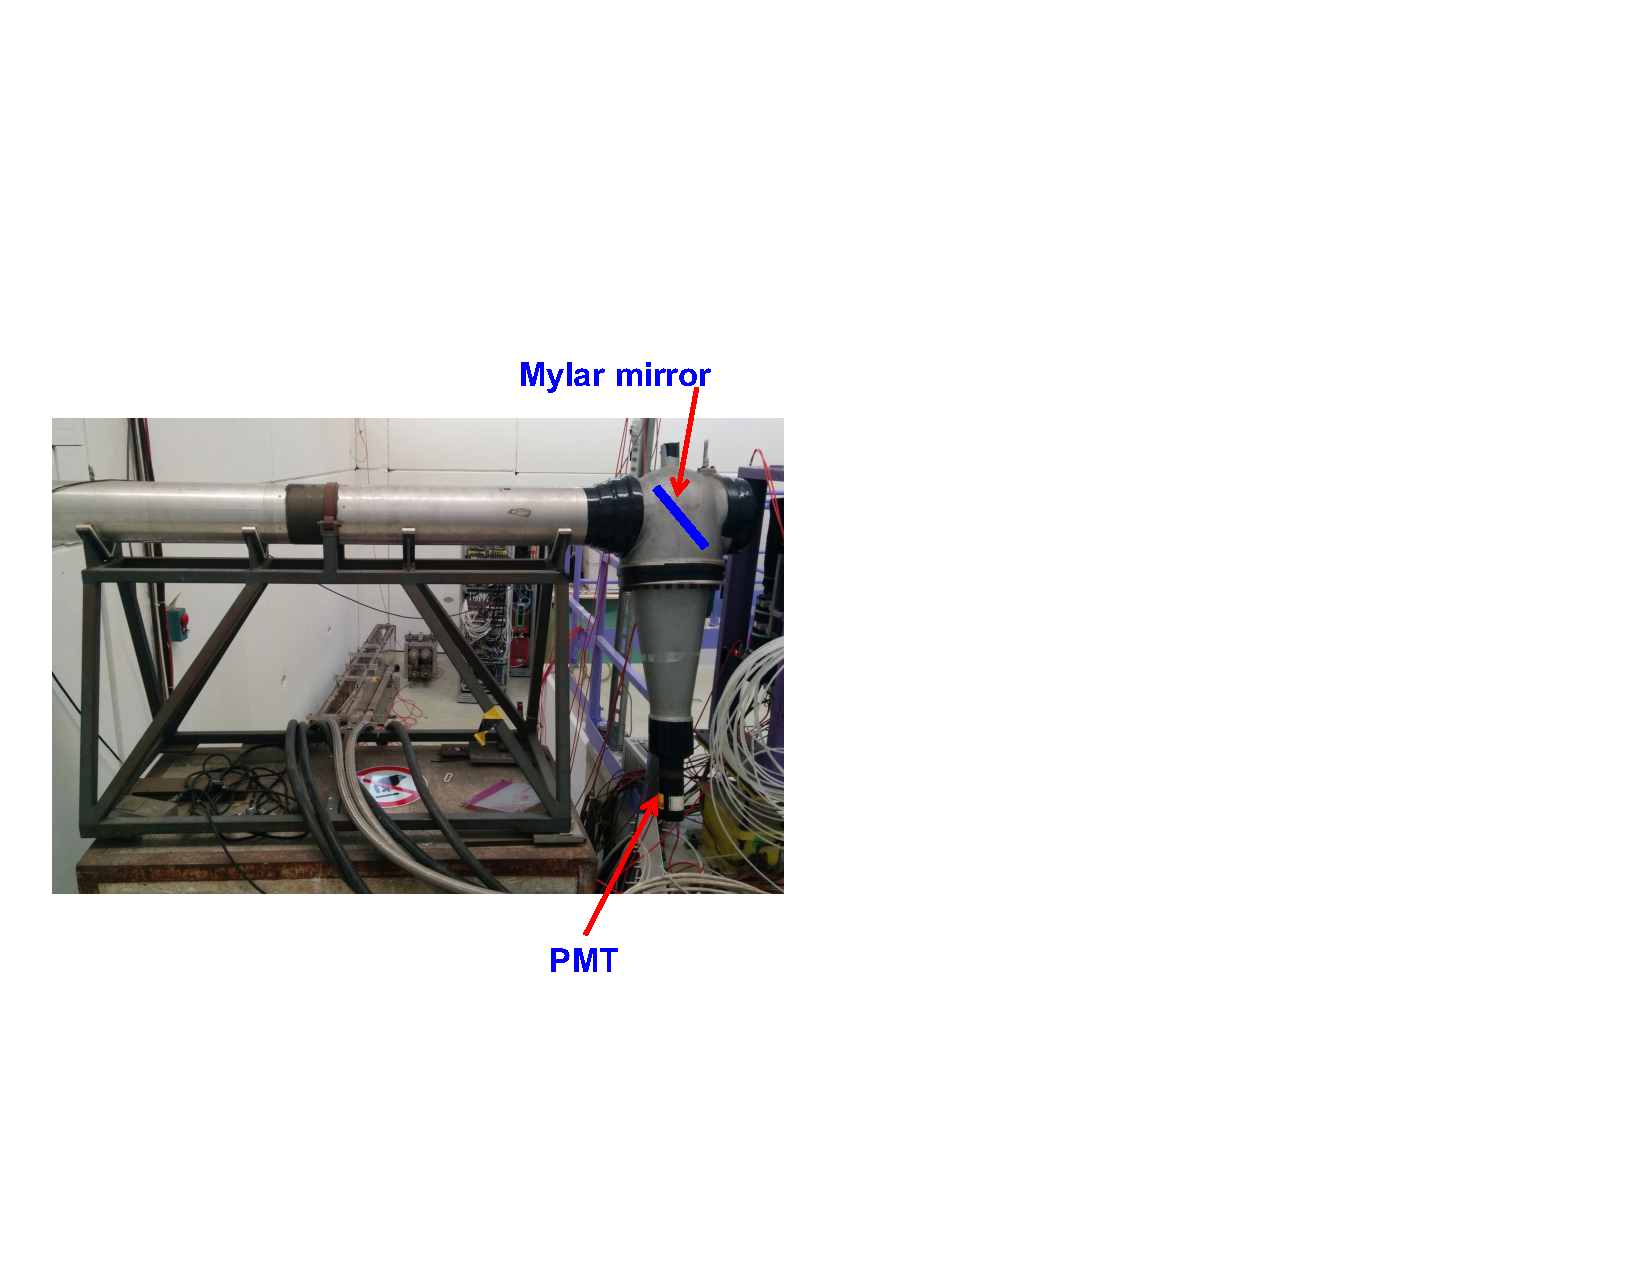
\includegraphics[width=0.65\textwidth]{beamline_ckv.pdf}
\end{cdrfigure}
\begin{cdrfigure}[Cherenkov gases]{ckv_gases}{Gas pressure threshold for the production of Cherenkov light for various particles as a function of particle momentum for Freon 12~\footnote{N. Charitonidis, Y. Karyotakis \it{et al.}, ``Hadron identification proposal for the ProtoDUNE experiments of CENF, to be published.} and CO$_2$ gases.}
  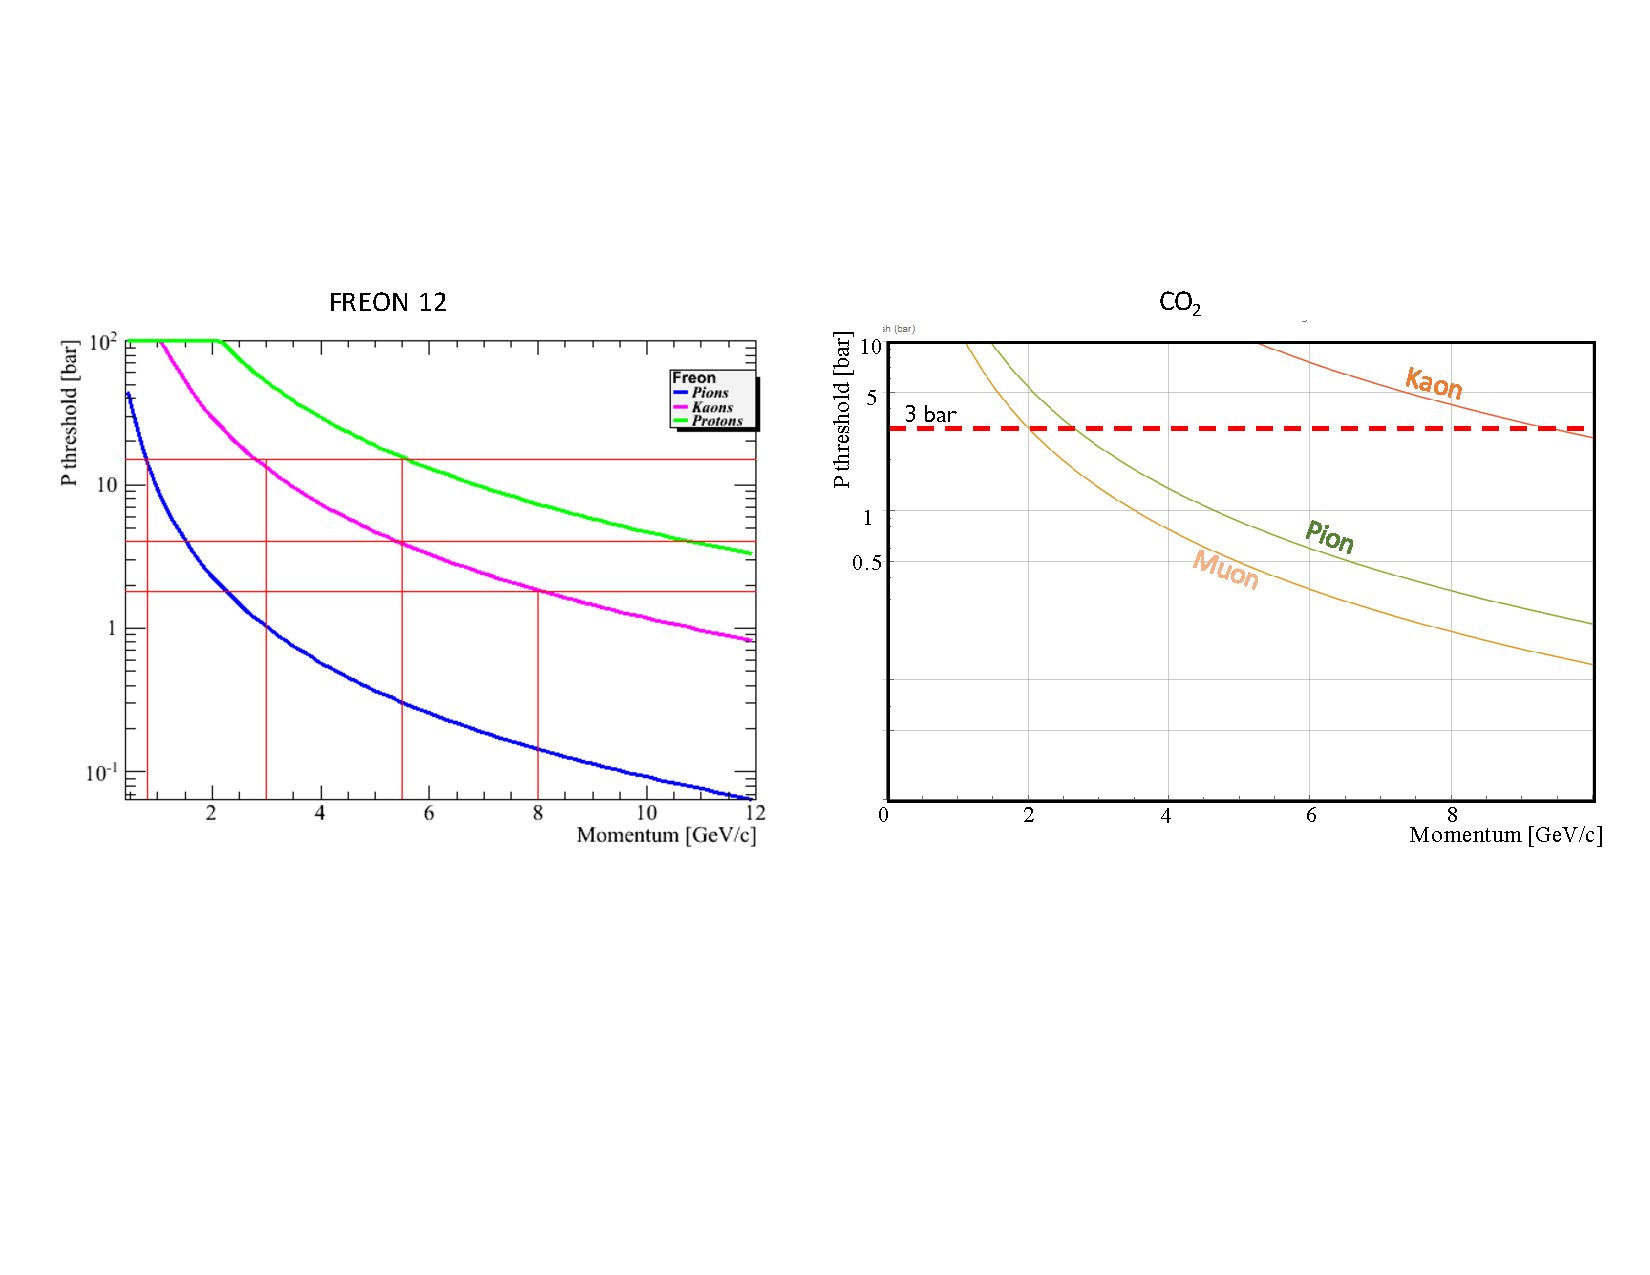
\includegraphics[width=0.99\textwidth]{beamline_CKVgases.pdf}
\end{cdrfigure}
Freon 12 has been selected for its high density, however,  to avoid liquefaction it cannot be operated at pressures larger than 3~bars.  CO$_2$ can be used more easily at higher pressures.  

 Figure~\ref{fig:ckv_gases} shows that pions can be tagged with a 3-bars Freon counter for momenta larger than 2~GeV/c, and kaons can be tagged with a high-pressure  (15-bars) CO$_2$  counter above 4~GeV/c.

The baseline plan for beam instrumentation includes a 2-m-long
Cherenkov  counter filled with Freon 12 at adjustable pressure up to
3~bars (XCET1), and a  2-m-long  
 Cherenkov  counter filled with CO$_2$ at adjustable pressure up to
 15~bars (XCET2).\\
%%
Existing Cherenkov counters at CERN are designed for pressures lower than  3~bar, therefore a new counter has to be manufactured in order to reach the 15~bars needed to efficiently tag kaons. Drawings for such high-pressure Cherenkov counters do exist, as they have been %since they were already 
used in the past. \\
%
Since it will not be necessary to use both counters at all energies, the CO$_2$
counter, filled at low pressure,  will be used for electron discrimination at beam momenta lower
than 4~GeV/c.  

A time-of-flight (ToF) system  is  necessary   to distinguish hadrons below the mentioned thresholds.
%
In summary:
\begin{itemize}
\item {\bf below 2~GeV/c} : one Cherenkov, filled with CO$_2$ at low
  pressure, discriminates electrons; ToF needed for hadrons.
\item {\bf 2-3~GeV/c} : one Cherenkov, filled with CO$_2$ low
  pressure, discriminates electrons; second Cherenkov, filled with
  Freon 12, tags pions; kaons are negligible.
\item {\bf 3-4~GeV/c} : one Cherenkov, filled with CO$_2$ at low
  pressure, discriminates electrons; second  Cherenkov, filled with
  Freon 12, tags pions; ToF is needed for kaon/proton discrimination
\item {\bf 4-7~GeV/c} : one Cherenkov, filled with CO$_2$ at high
  pressure, tags kaons; second  Cherenkov, filled with
  Freon 12, tags pions; electron content of the beam is low and can be
  discriminated by reconstruction.
\end{itemize}

  From table \ref{tab:beampartcomp} it is evident that the kaon content of the beam is negligible at least below 2~GeV/c, thus  only pion-proton separation is needed at low energies. Figure~\ref{fig:toftau} shows the ToF resolution needed to distinguish among particle species at the $4\sigma$ level as a function of the particle momentum, assuming a 23-m-long path. To distinguish pions from protons below 2~GeV/c, a 1-ns resolution is enough, while 300~ps are necessary for kaon-proton distinction up to  4~GeV/c. It should also be noted that a ToF system with a $\sim$100-ps resolution would allow identification of protons from other hadrons up to 7~GeV; this would preclude the need for a % so that the 
  high-pressure CO$_2$ Cherenkov. %could be avoided. 
  Conversely, covering %in order to cover 
  the full energy range up to 7~GeV for all hadron  types would require a ToF system with a resolution better than 40~ps. % would be needed.
In the following, two (possibly complementary) ToF systems are described.
\begin{cdrfigure}[Required ToF resolution]{toftau}{Required ToF resolution to  distinguish among particle species at the $4\sigma$ level as a function of the particle momentum, assuming a 23~m long path. }
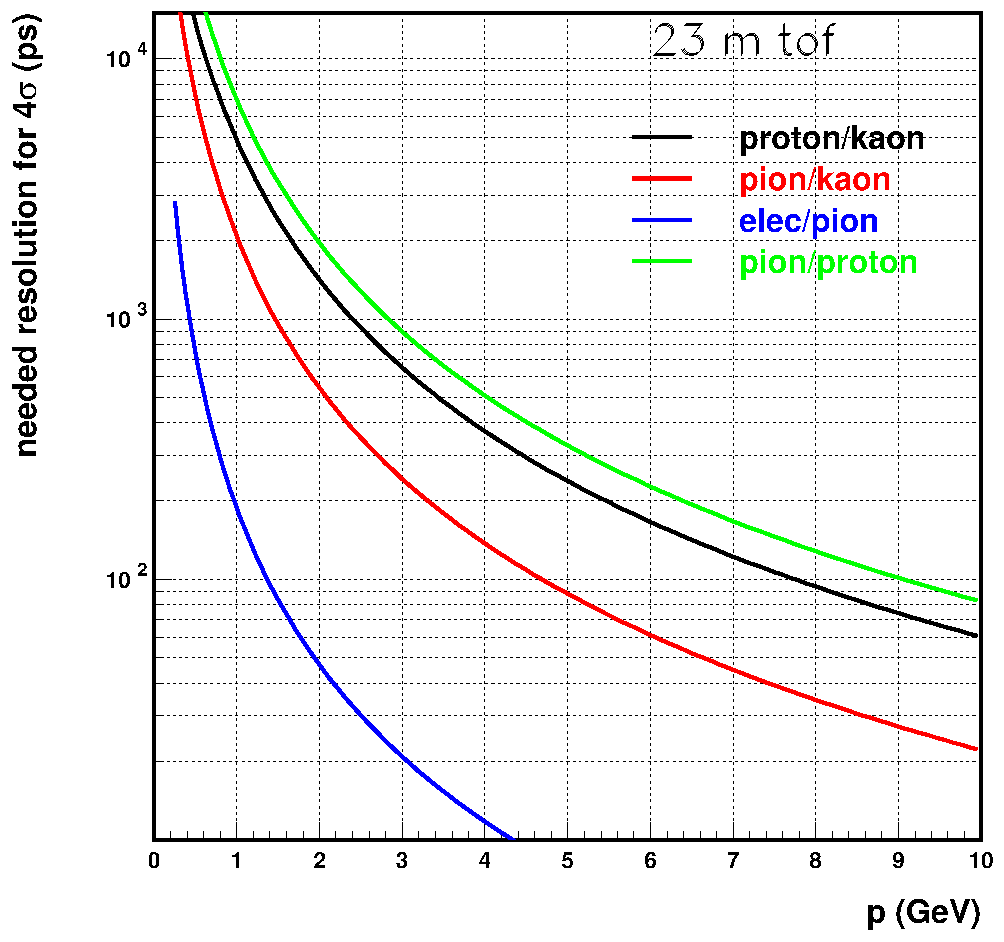
\includegraphics[width=0.65\textwidth]{toftaulow.pdf}
\end{cdrfigure}

\paragraph{pLAPPD Time-of-flight system}
Fermilab is testing a ToF system that would utilize %a 
6 $\times$ 6-cm$^2$
large-area picosecond photodetectors (pLAPPDs), as shown in Figure \ref{fig:pLAPPD}.
 The microchannel plates based devices
are capable of $< 50$-ps resolution with gains of $10^6-10^7$,
mm position resolution along one axis, and slightly worse resolution
along the other axis.  The photodetector is mounted on a readout
board, and the relevant exterior dimensions are 165.1~mm $\times$ 109.3~mm and a
thickness of 16~mm. The active area is defined by the four squares visible in Figure \ref{fig:pLAPPD}, and amounts to about 8~cm$^2$. Tests of these devices in the LAriat beam are underway, to precisely assess the timing capabilities. \fixme{Any citation to add?}
\begin{cdrfigure}[pLAPPD]{pLAPPD}{Photo of one pLAPPD device as proposed for the H2 and H4 beamlines.}
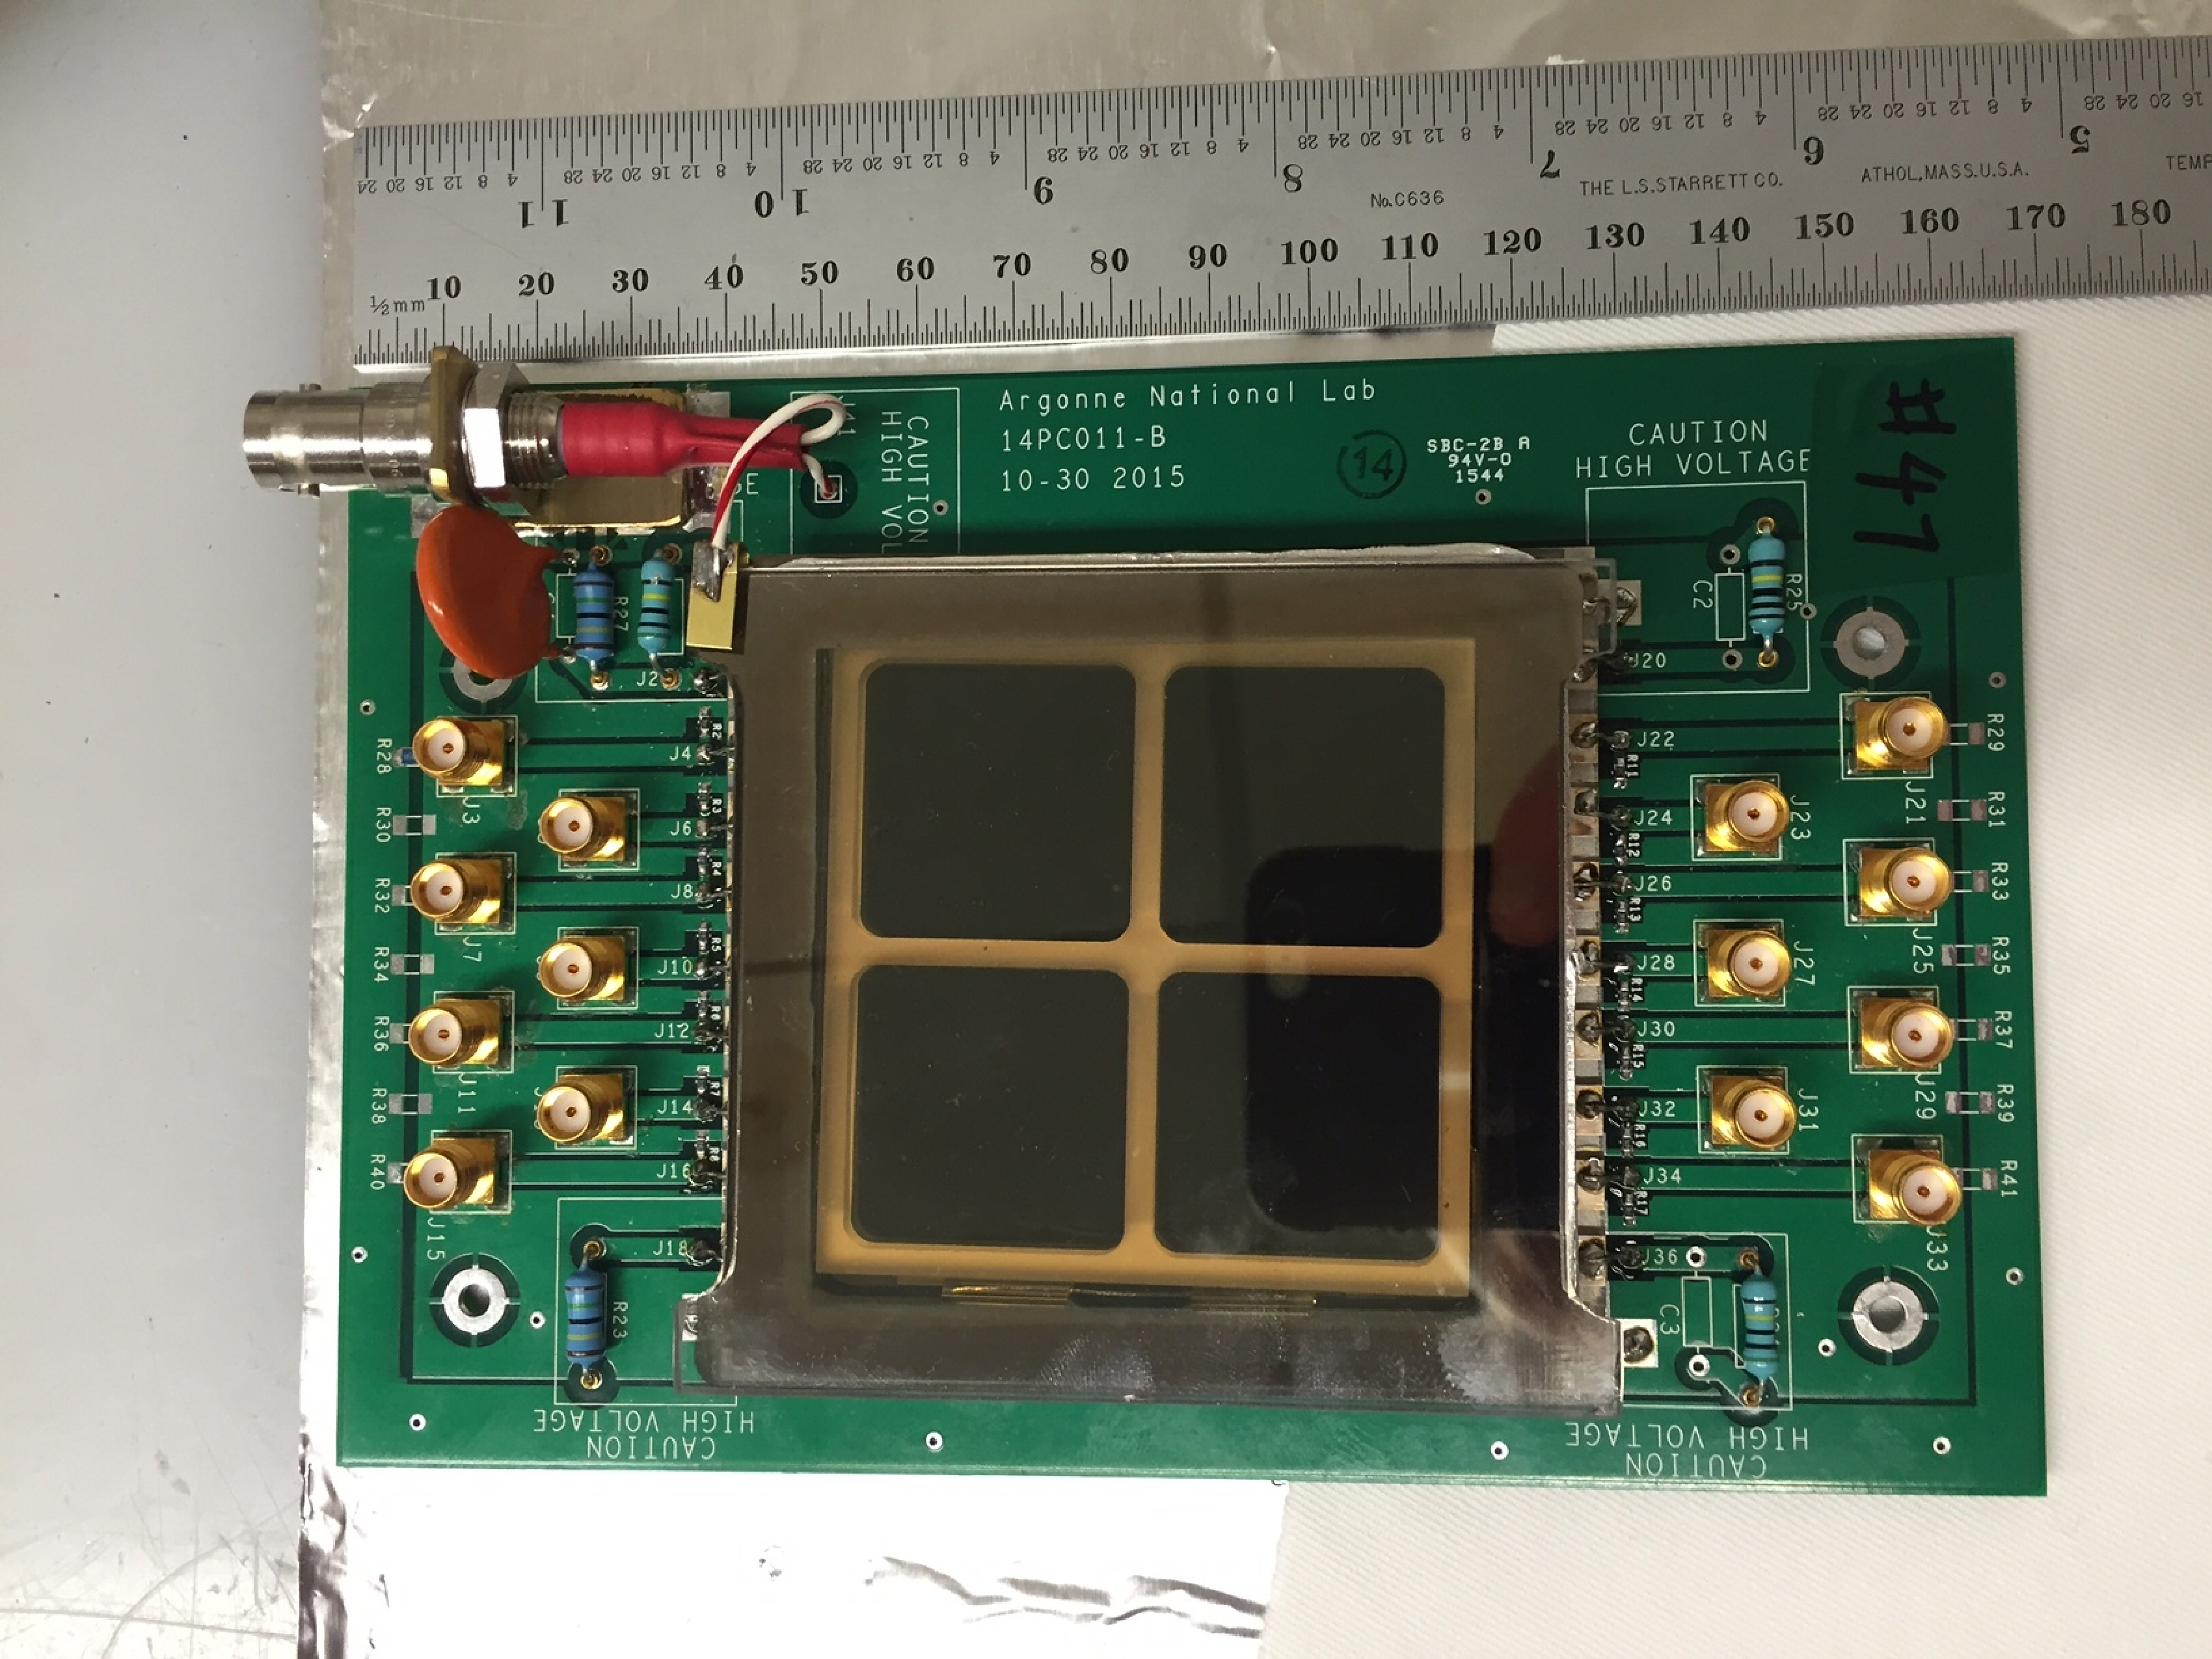
\includegraphics[width=0.65\textwidth]{LAPPD.pdf}
\end{cdrfigure}

\paragraph{Alternative Time-of-flight system}
The  scintillating-fiber monitors can be used also for ToF purposes with the goal of a 1-ns timing resolution, suitable for low momentum ($<$ 2 GeV/c) beams. 
The idea is to read out the detectors with the STiC ASIC~\cite{STIC} for SiPM readout. \fixme{Is STiC defined?}
%%%, developed at the  Kirchhoff Institute for Physics in Heidelberg - will be clear from reference
In this configuration, the time resolution would be dominated by the fiber response. Monte Carlo simulations estimate a resolution better than 1~ns. 
A small prototype will be built and tested in the next few months to fully validate this solution.

%%%%%%%%%%%%%%%%%%%%%%%
\subsection{Material budget and discussion}
\label{beam-material-budget}

The choice of ToF system, and the actual configuration of the beamline at different beam momenta  depend also on the material budget. 
\fixme{Please define `material budget'. I think it relates to how much material is in the beam's path, but not precisely sure. Anne}
As described in the following, some of the instrumentation will have to be removed, or at least emptied, when operating below $\approx$~2 GeV. Also, the ToF system will be different for the low-energy range.

Summarizing %ing up all 
the required instrumentation, the ``full'' beamline will  include
 five beam monitors (two for tracking and three for spectrometry), two ToF devices, and two 2-m-long Cherenkovs at high density or pressure. The material budget would be much too high for operation at low momenta (below 2~GeV/c),  and in general for operation with electron beams.  
A full FLUKA\cite{fluka05,Fluka15}  simulation of materials in the beamline and of the ProtoDUNE-SP detector, including the beam window details, has been used to evaluate the effect of materials; it is presented here. 
%\fixme{Should also mention that a second simulation was performed using GEANT 4 and that consistent results were obtained. }
%\fixme{ I saw no GEANT4 simulation with the beam instrumentation, except the one, very recent, from Nikos. And I would like to keep the ``materials etc'' simulations on the Protodune side, not on the Beam group. Conversely, I saw at the workshop strange GEANT4 results with a wrong geometry of the beam window. If you refer to the old work done last year, the materials have changed.}
Earlier material studies with FLUKA have been compared with GEANT4-based results and good agreement was found. More recent GEANT4-based studies are still in progress.

Since the final layout of the beamline optics was delivered only recently, the simulations presented here assume a straight line with an initially parallel beam, deflected only by scattering. Particles are assumed to be ``lost'' when scattered outside of the beam pipe. Inclusion of the beamline's magnetic elements is underway. 
 Figure~\ref{fig:matblfull} shows the evolution of the material budget with a full instrumentation, assuming pLAPPD for ToF. The total, including the beam window, would add $0.6X_0$, 0.15 interaction lengths, and an energy loss for a mip of 28~MeV.

The largest energy-loss contribution comes from the Cherenkov detectors and from the  ToF system. Cherenkovs are not particularly useful for low energies (except a low-pressure one for electron discrimination), and can be easily removed from the beamline and either substituted with a section of vacuum pipe, or emptied.  
In a configuration %situation 
without Cherenkovs, the pLAPPD devices plus monitors would still account for almost  $0.2X_0$. Besides energy degradation, scattering of low-energy particles would  further degrade the pion and proton content of the beam.  Figure~\ref{fig:1GeVtof} shows examples of the beam degradation due to materials at 1~GeV/c; the rate of pions arriving at the detector is reduced by a factor of 2.5, and the energy spread rises to 1.2\%. The rate of protons stopping in the detector is reduced by a factor of 4, and the energy spread amounts to 2\% rms. This calculation is done in optimistic conditions, i.e., neglecting the efficiency loss due to the small active area of the pLAPPD devices.
%
To overcome this problem, it is foreseen to use scintillating fibers as ToF devices for the lowest-energy beams (<2~GeV), and pLAPPD above 2~GeV.
   This will require reconfiguration of the beamline, and needs to be carefully considered in the run plan, but is known to be feasible. %it is feasible.  

It should also be noted that good enough performance of the (combined) ToF system could preclude the need for high-pressure  Cherenkov counters. 
%a good performance of the (combined) ToF system could avoid the use of high pressure  Cherenkov counters. 
This option is not considered here, but %could represent an important simplification in case
\fixme{``could simplify the configuration, and can be considered if'' }
 the pLAPPD tests demonstrate a resolution of $\approx$20ps.

  \begin{cdrfigure}[Material budget]{matblfull}{Material budget in the beamline, as a function of the distance from the center of the detector (in cm). The red line describes the amount of $X_0$, the black line the amount of interaction length, both read on the left axis. The black dotted line is the average energy lost by a mip particle, and is read on the right axis (in MeV). Vertical lines show the positions of the various beam monitors (in between the two blue lines are the 3 devices for spectrometry, ``bm'' is the last beam monitor, ``bw'' is the starting point of the beam window).}  
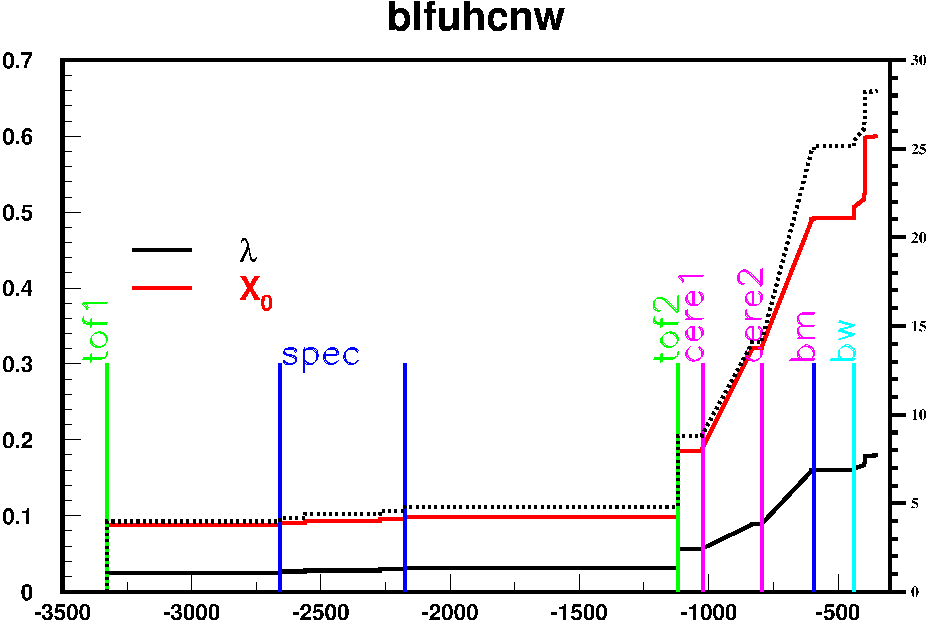
\includegraphics[width=0.65\textwidth]{blfuhcnwrayplo.pdf}
\end{cdrfigure}
%
 \begin{cdrfigure}[Effect of materials at  1GeV]{1GeVtof}{Effect of materials at  1GeV/c. Left: $\pi$ beam, energy of the particle entering in the detector, in three conditions: with  beam monitors, with beam monitors and pLAPPD for ToF, with the whole beamline filled with air (and no instrumentation). Right: proton beam, energy deposited by protons stopping in the LAr active volume, in three conditions: without instrumentation (the beam window is always present), with the scintillators only, and with scintillators plus pLAPPD for ToF.}
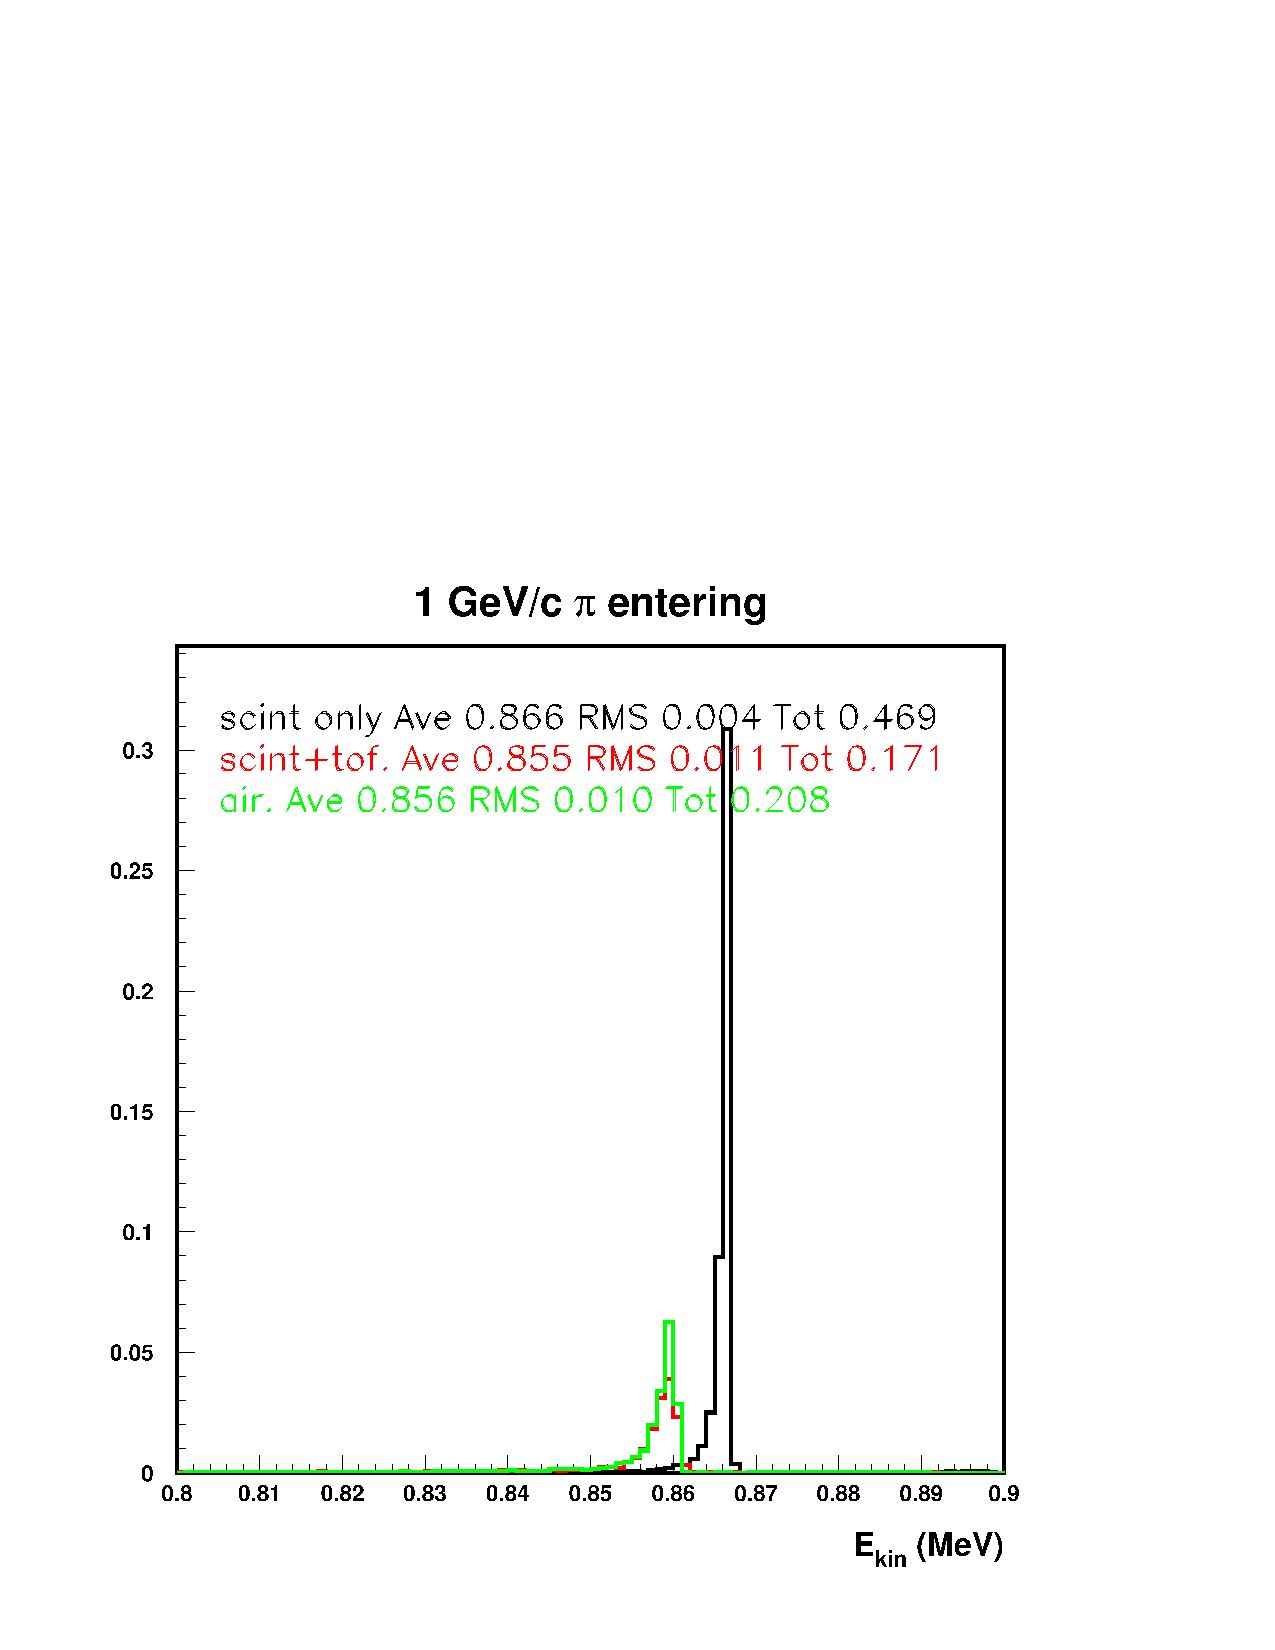
\includegraphics[width=0.45\textwidth]{pi1p0gev_innw.pdf}
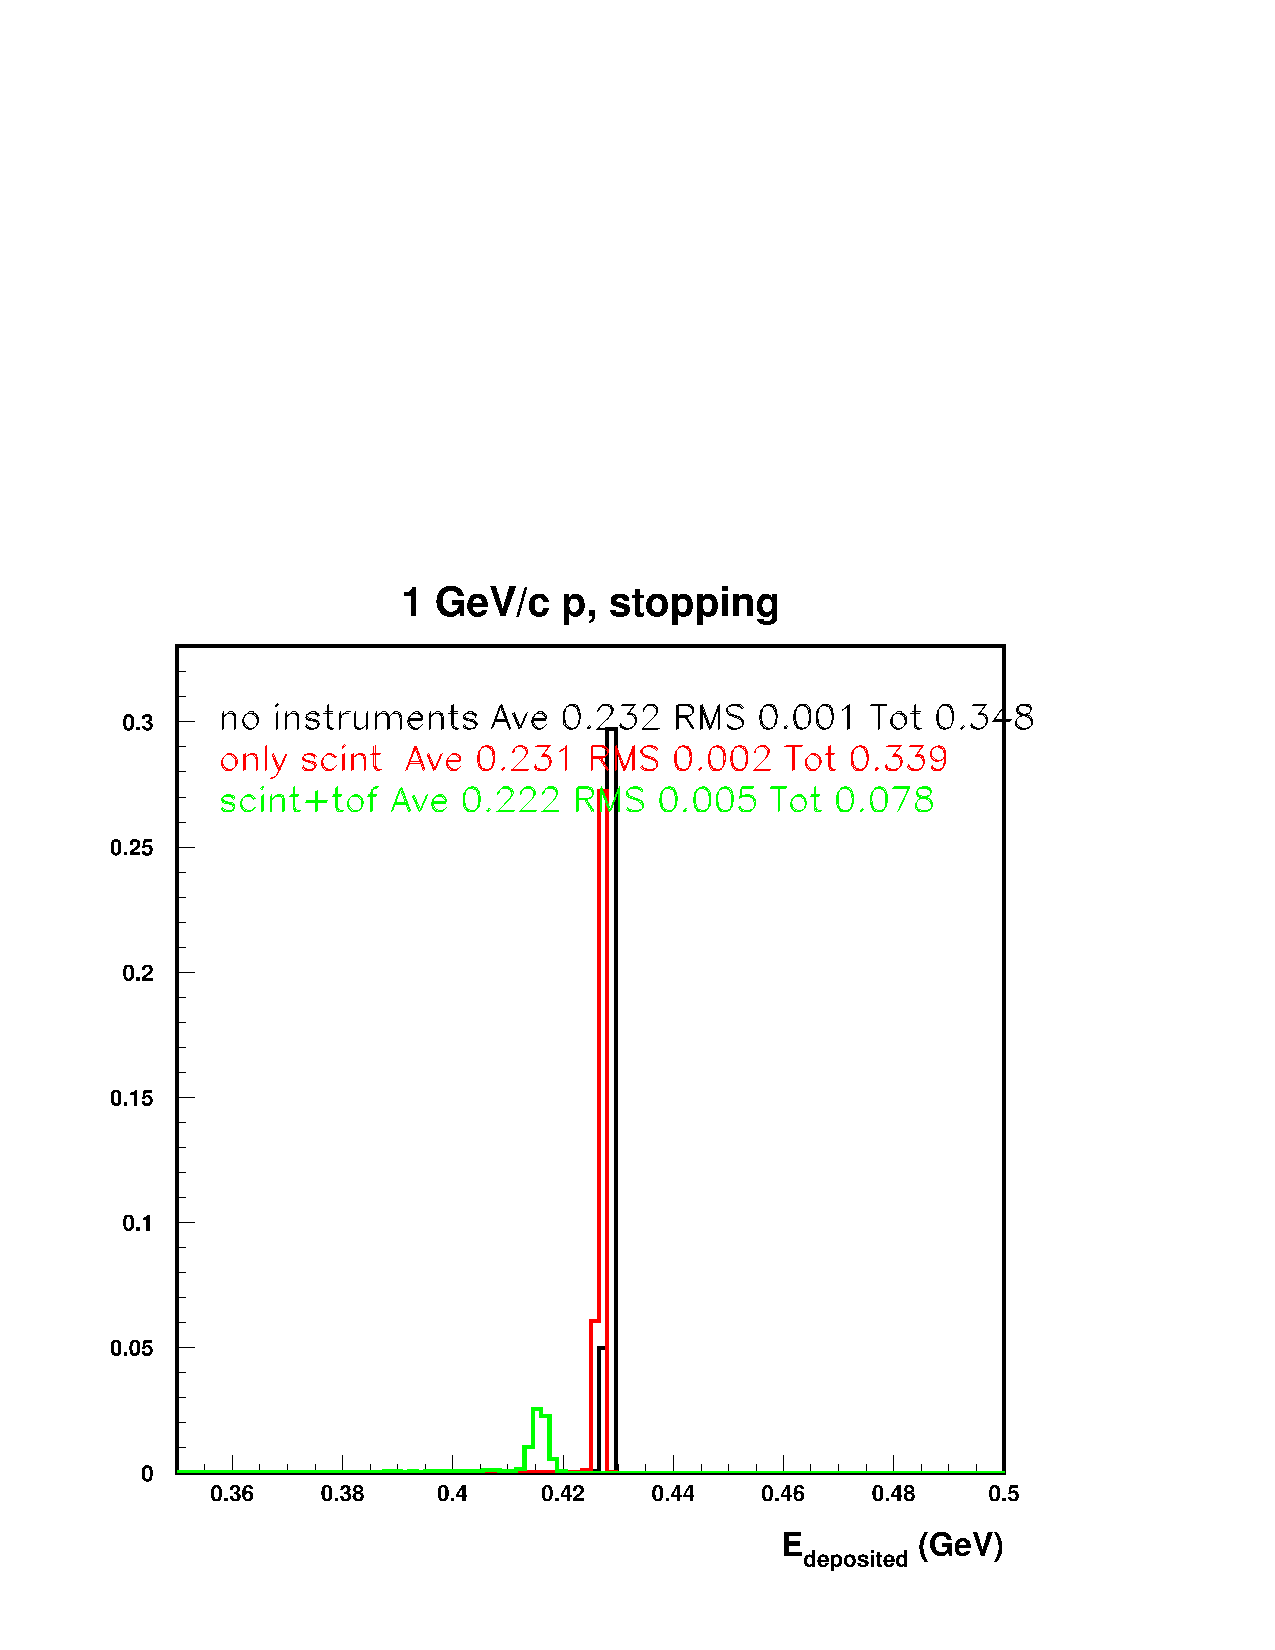
\includegraphics[width=0.45\textwidth]{p1gevstopnoqnw.pdf}
\end{cdrfigure}



%%%%%%%%%%%%%%%%%%%%%%%
\subsection {Trigger and data acquisition}

The beam instrumentation will provide a trigger signal, built from the coincidence of the two last beam monitors, vetoed by the electron-tagging Cherenkov for low-energy beams. 
\fixme{``The beam instrumentation will provide a trigger signal, built from the coincidence of the two last beam monitors. For low-energy beams, the electron-tagging Cherenkov will provide a veto.''? (otherwise it makes reader wonder about everything besides low-energy)}  
A trigger mask, providing the status of the other counters, will also be provided. 
 Synchronization of the detector data acquisition (DAQ) with the beam instrumentation DAQ will be ensured by a common time stamp through a White Rabbit network.
 White Rabbit is a fully deterministic Ethernet-based network for general purpose data transfer and synchronization. It can synchronize over 1000 nodes with sub-ns accuracy over fiber lengths of up to 10~km. It is developed and widely used at CERN.  \fixme{citation recommended}

Beam instrumentation data will be read out independently on a separate DAQ stream. However,  
the beam data fragments corresponding to  events with a valid trigger from both beam and ProtoDUNE-SP will be merged online with the detector data.
 
